\chapter{Results and Discussion}
\label{sec:results}

We evaluated the in chapter \ref{chapter:alphalinkage} proposed algorithms with the in chapter \ref{chapter:datasets} discussed datasets aiming to find new subcategories for the text data and to generate better clusterings overall. The quality of the clusterings was calculated with the in chapter \ref{chapter:costfunctions} explained cost functions.

\section{Clustering Text Data}

We subsampled the NELL data to a maximum of 250 points in each class and then evaluated each of the 32 classes separately. Figure \ref{fig:nellresults} shows the resulting majority distances for the three different types of linear interpolation.

\begin{figure}[h]
\centering
\begin{minipage}{.3\textwidth}
  \centering
  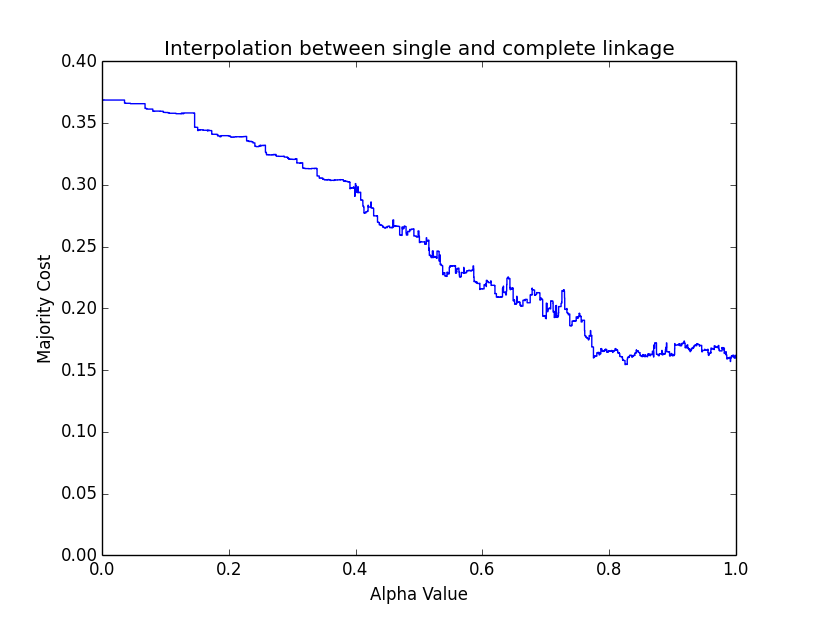
\includegraphics[width=\linewidth]{images/nell_sc}
\end{minipage}
\begin{minipage}{.3\textwidth}
  \centering
  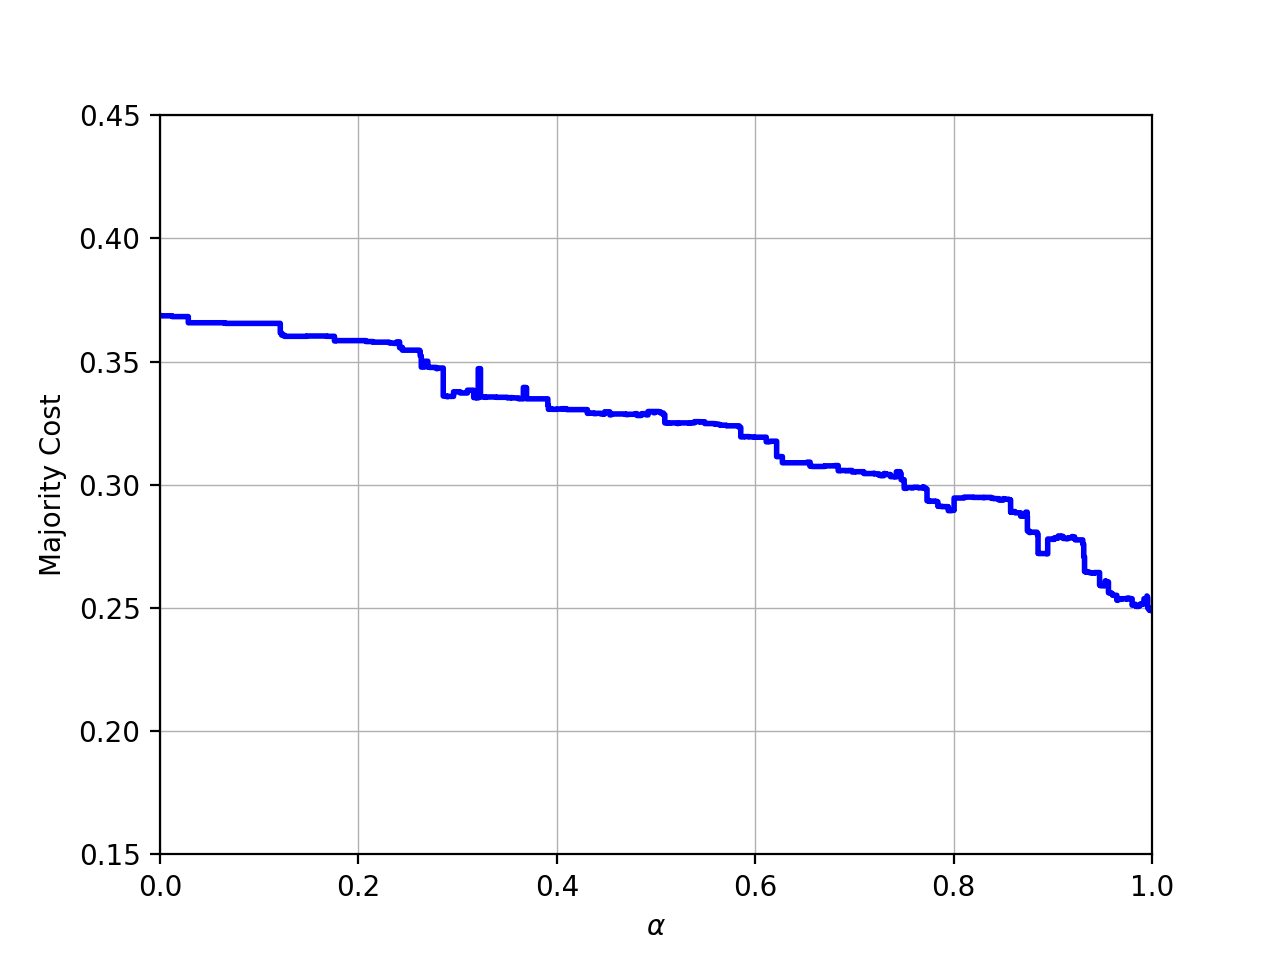
\includegraphics[width=\linewidth]{images/nell_sa}
\end{minipage}
\begin{minipage}{.3\textwidth}
  \centering
  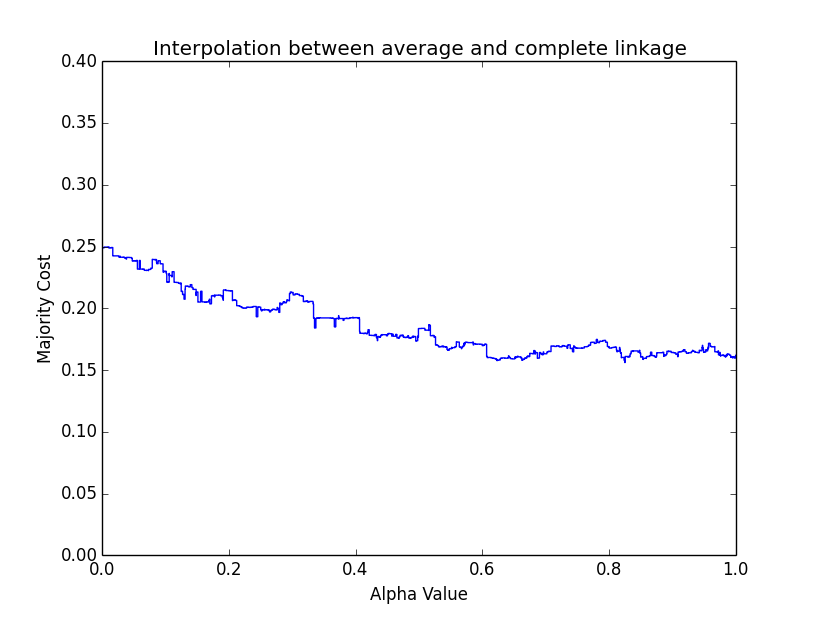
\includegraphics[width=\linewidth]{images/nell_ac}
\end{minipage}
\caption{The omniglot dataset contains handwritten characters of different alphabets, such as Latin, Greek and Hebrew \cite{Lake1332}.}
\label{fig:nellresults}
\end{figure}

We observe that single linkage performs very poorly and complete linkage performs very well for the NELL data. Table \ref{table:nellresults} shows the improvements we got over the other clustering strategies.

\begin{table}[h]
    \centering
    \begin{tabular}{|l | l|}
    \hline
    Strategy & Majority Cost\\ \hline
    Single Linkage & 0.36871\\
    Average Linkage & 0.248913\\
    Complete Linkage & 0.15935\\
    $\alpha_{SC}(0.825)$ & 0.15442\\
    $\alpha_{AC}(0.825)$ & 0.15569\\\hline
    \end{tabular}
    \caption{Our proposed algorithm reduces the cost by $\Delta cost = 0.493\%$.}
    \label{table:nellresults}
\end{table}

The total improvement over the common linkage methods is $0.493\%$ and the best clustering we generated had an error of $15.442\%$. With this clustering we also managed to extract new subcategories as listed in table \ref{table:nellcategories}.

In addition to averaged costs, we also evaluated the clusterings for multiple values of $\alpha$. This is helpful in situations where a domain expert can select from multiple suggestions. For example, if we consider the best three values of $\alpha$, the domain expert can choose from three different clusterings. In order to calculate the $N$ best values of $\alpha$, we selected the 32 optimal values resulting from the experiments that led to an integer optimization problem. This resulted in ?????.

As our only formal guarantee was that there will be a maximum of $O(n^8)$ intervals in the range between single and complete linkage, we also had a look at the actual results. Since the proof for single and complete linkage in Balcan et. al \cite{DBLP:journals/corr/BalcanNVW16} relies on the fact that the distance $d_{SC}(X,Y,\alpha)$ is based on four points and a split between two merges thus is based on eight points, we would expect experiments containing average linkage to have more intervals, because the average linkage distance is based on all points of the clusters. Finding formal guarantees for the average distance is not a part of this thesis and will briefly be discussed in section \ref{section:futurework}.

In addition to looking at the resulting loss, we also evaluated how well our algorithm is able to discover new subcategories. In the given data, only very specific class labels are given such as luxurious suites, broad road or denver international airport that all belong to a certain location, i.e. these noun phrases have the specific label and the only more generalized group is the location class. In \ref{sec:nellsubcategories}, we listed potential subcategories that our algorithm found and annotated them with a label manually. For instance, the noun phrase luxurious suites could then be grouped together with similar ones into the cluster suite that is a subset of the cluster office building room.

\section{Clustering Image Data}

We first clustered the MNIST data. First experiments were run with 250 points in each run.

\begin{figure}[h]
\centering
\begin{minipage}{.3\textwidth}
  \centering
  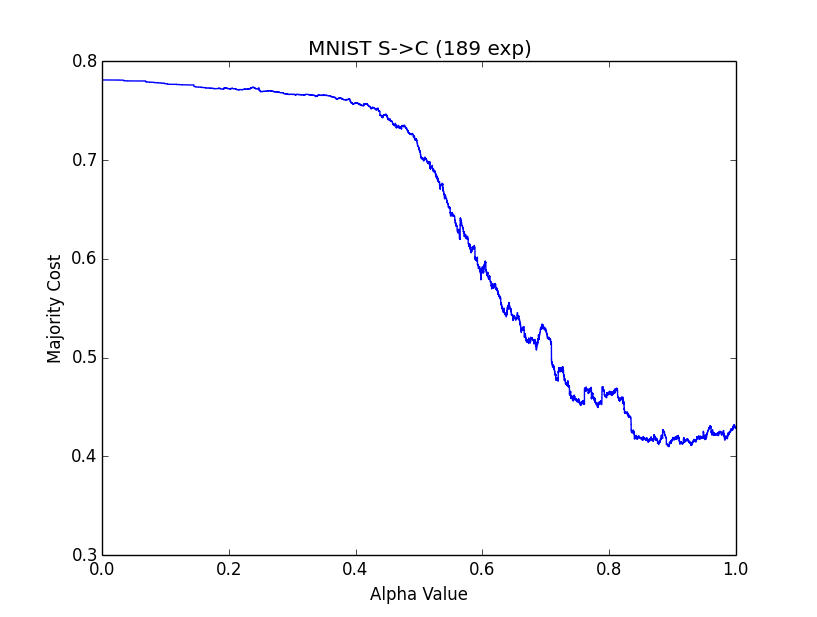
\includegraphics[width=\linewidth]{images/MNIST_SC_250}
\end{minipage}
\begin{minipage}{.3\textwidth}
  \centering
  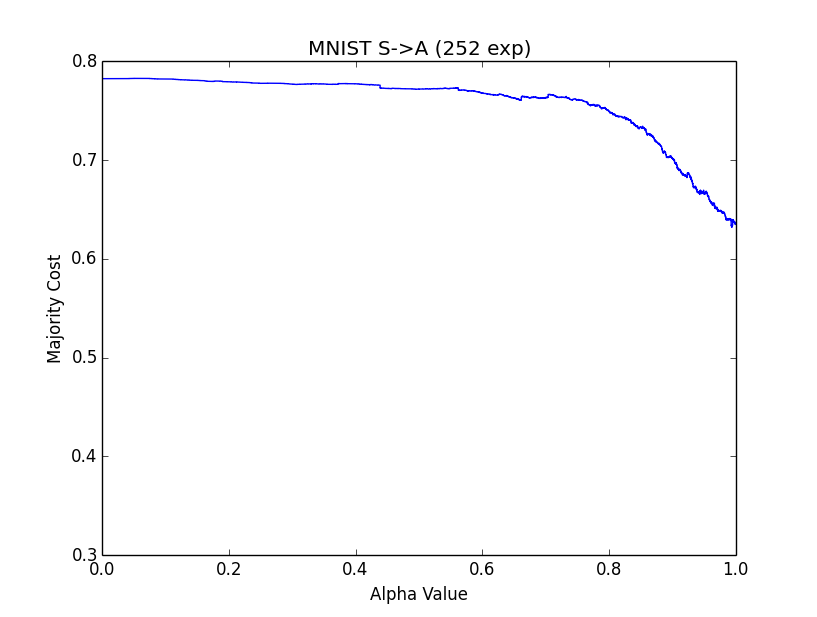
\includegraphics[width=\linewidth]{images/MNIST_SA_250}
\end{minipage}
\begin{minipage}{.3\textwidth}
  \centering
  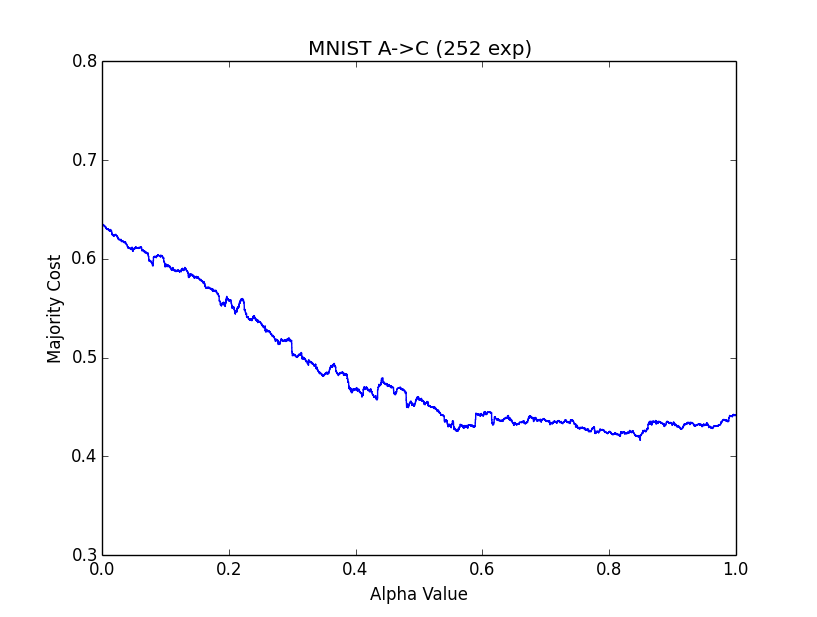
\includegraphics[width=\linewidth]{images/MNIST_AC_250}
\end{minipage}
\caption{The omniglot dataset contains handwritten characters of different alphabets, such as Latin, Greek and Hebrew \cite{Lake1332}.}
\label{fig:mnist250}
\end{figure}

Figure \ref{fig:mnist250} shows the experimental results averaged over all 252 $10 \choose 5$ experiments, i.e. all different combinations of five unique labels. Again, we observe that interpolating between single and average linkage does not give us good results. Table \ref{table:mnist250results} summarizes the results we obtain for these experiments.

\begin{table}[h]
    \centering
    \begin{tabular}{|l | l|}
    \hline
    Strategy & Hamming Cost\\ \hline
    Single Linkage & 0.782354\\
    Average Linkage & 0.634206\\
    Complete Linkage & 0.441931\\
    $\alpha_{SC}(0.861624,)$ & 0.420714\\
    $\alpha_{AC}(0.849407)$ & 0.416627\\\hline
    \end{tabular}
    \caption{Our proposed algorithm reduces the cost by $\Delta cost = 2.5304\%$.}
    \label{table:mnist250results}
\end{table}

Reducing the cost by $\Delta cost = 2.5304\%$ seems to be a good result already. However the goal was to learn a parameter $\alpha$ that represents the entire dataset well. Because the procedure is very ressource-expensive, the results only looked at the first 500 points of the dataset as we clustered points from five labels in experiments of 250 points, i.e. we were using the first 50 points for each of the ten labels. This led us to running the same setting with other batches of the dataset to see if the subset of 500 points gives a good representation of the entire dataset. Figure ??? shows the results for the second batch and unfortunately the curves look quite differently, i.e. the batch did not give a good representation for the dataset.

To overcome this problem, we decided to scale up the experiments, so each of them used 1,000 instead of 250 points. As we used cloud computing to run the experiments in a reasonable time, we only evaluated the single to complete linkage and the average to complete linkage interpolation. We started with the single to complete linkage interpolation, where we show the results for the first six batches in figure \ref{fig:mnist1000sc}. Each batch contains 2,000 points, i.e. the six batches cover the first 12,000 points of the dataset.

\begin{figure}[h]
\centering
\begin{minipage}{.3\textwidth}
  \centering
  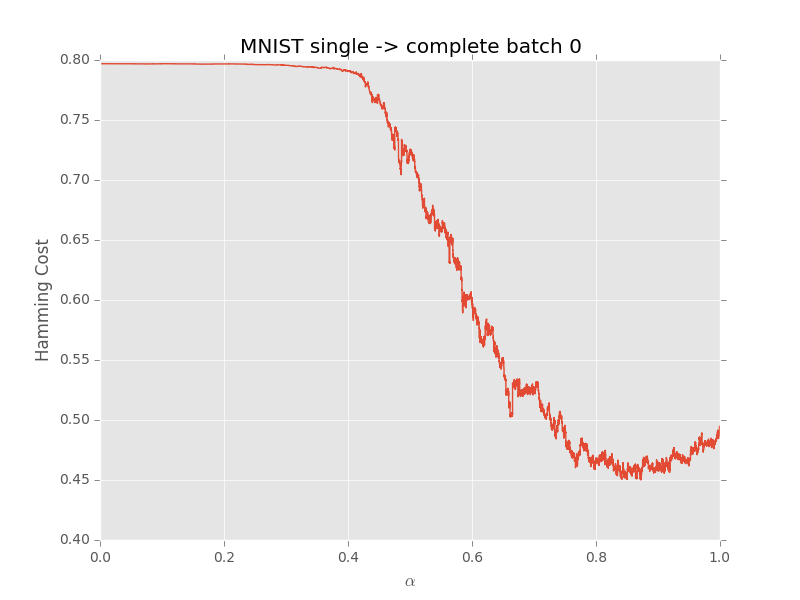
\includegraphics[width=\linewidth]{images/mnist-sc-0}
\end{minipage}
\begin{minipage}{.3\textwidth}
  \centering
  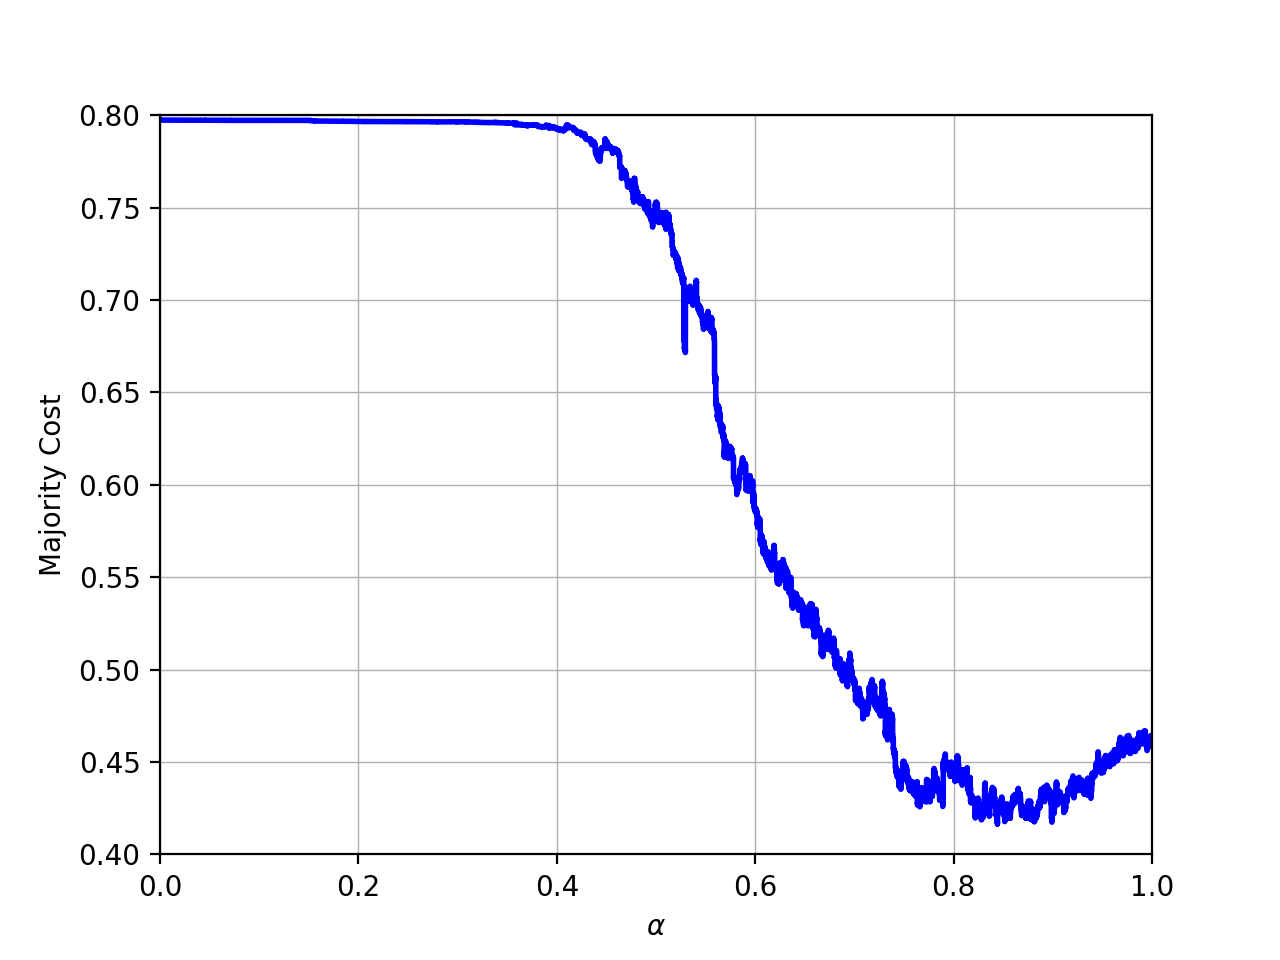
\includegraphics[width=\linewidth]{images/mnist-sc-1}
\end{minipage}
\begin{minipage}{.3\textwidth}
  \centering
  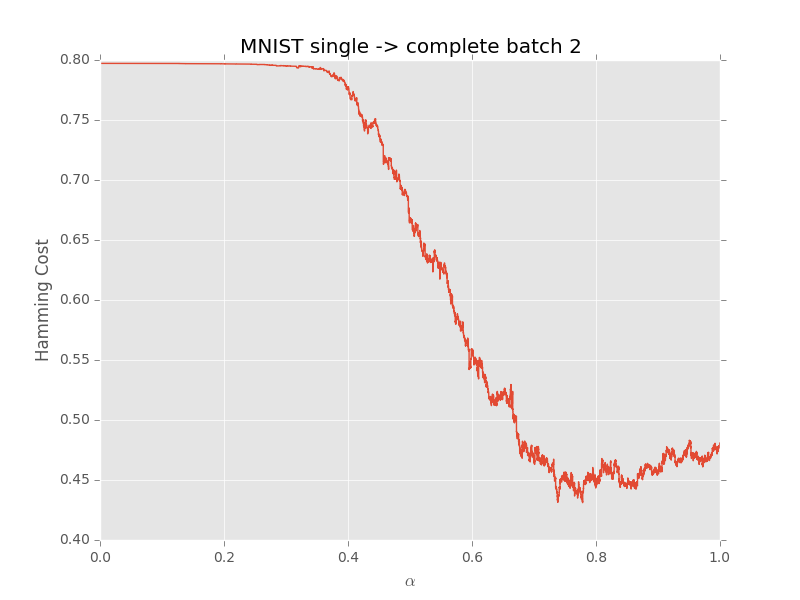
\includegraphics[width=\linewidth]{images/mnist-sc-2}
\end{minipage}
\begin{minipage}{.3\textwidth}
  \centering
  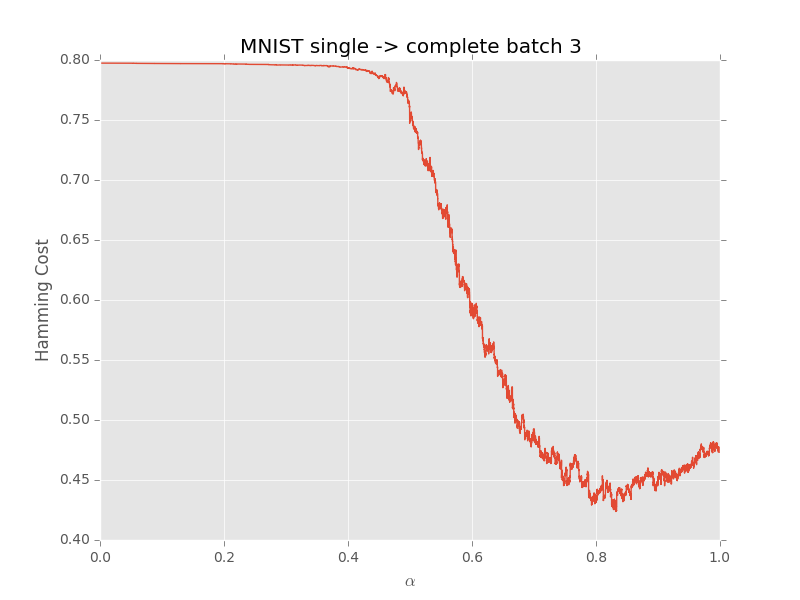
\includegraphics[width=\linewidth]{images/mnist-sc-3}
\end{minipage}
\begin{minipage}{.3\textwidth}
  \centering
  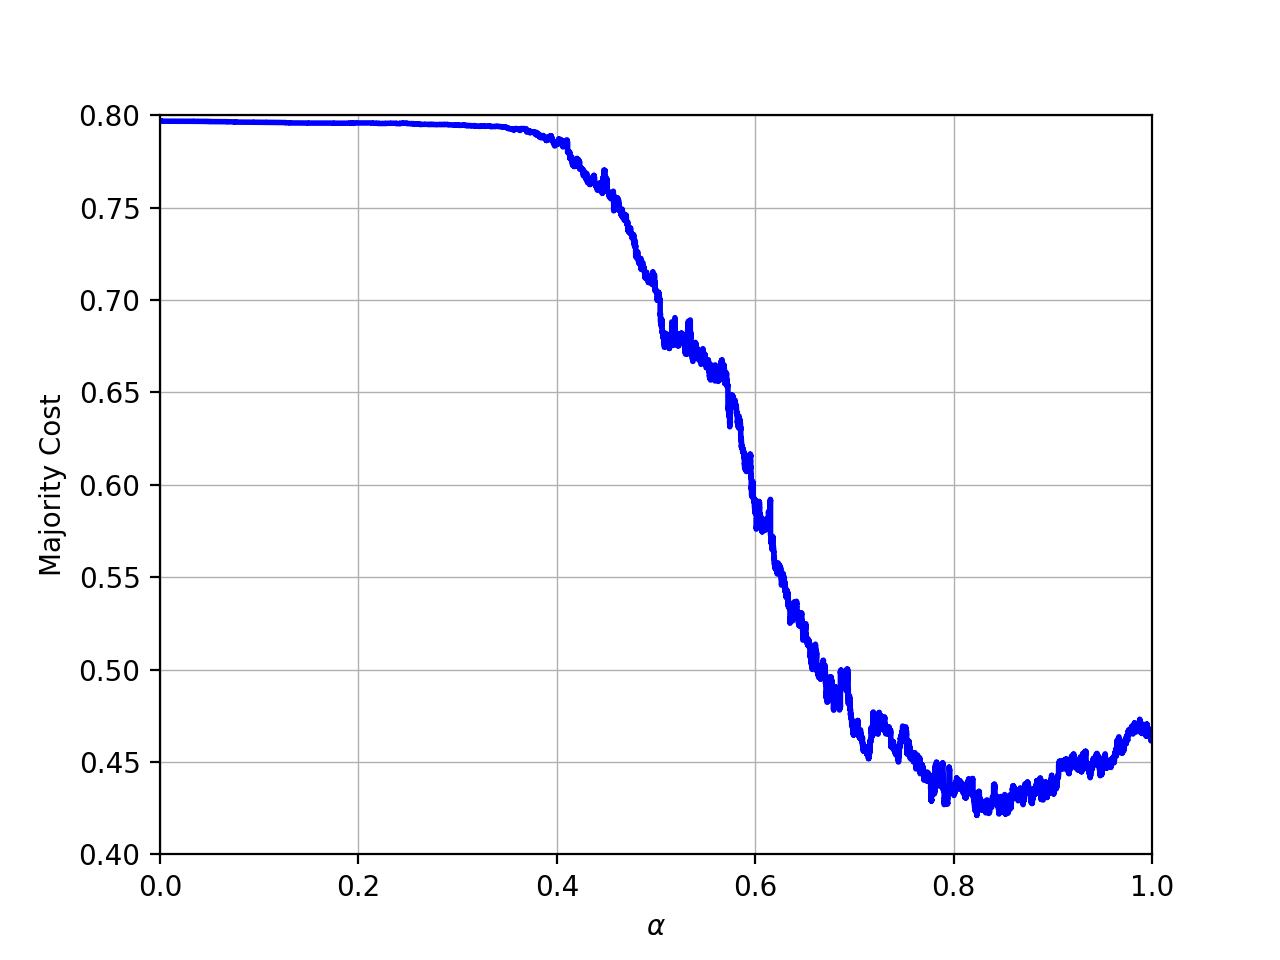
\includegraphics[width=\linewidth]{images/mnist-sc-4}
\end{minipage}
\begin{minipage}{.3\textwidth}
  \centering
  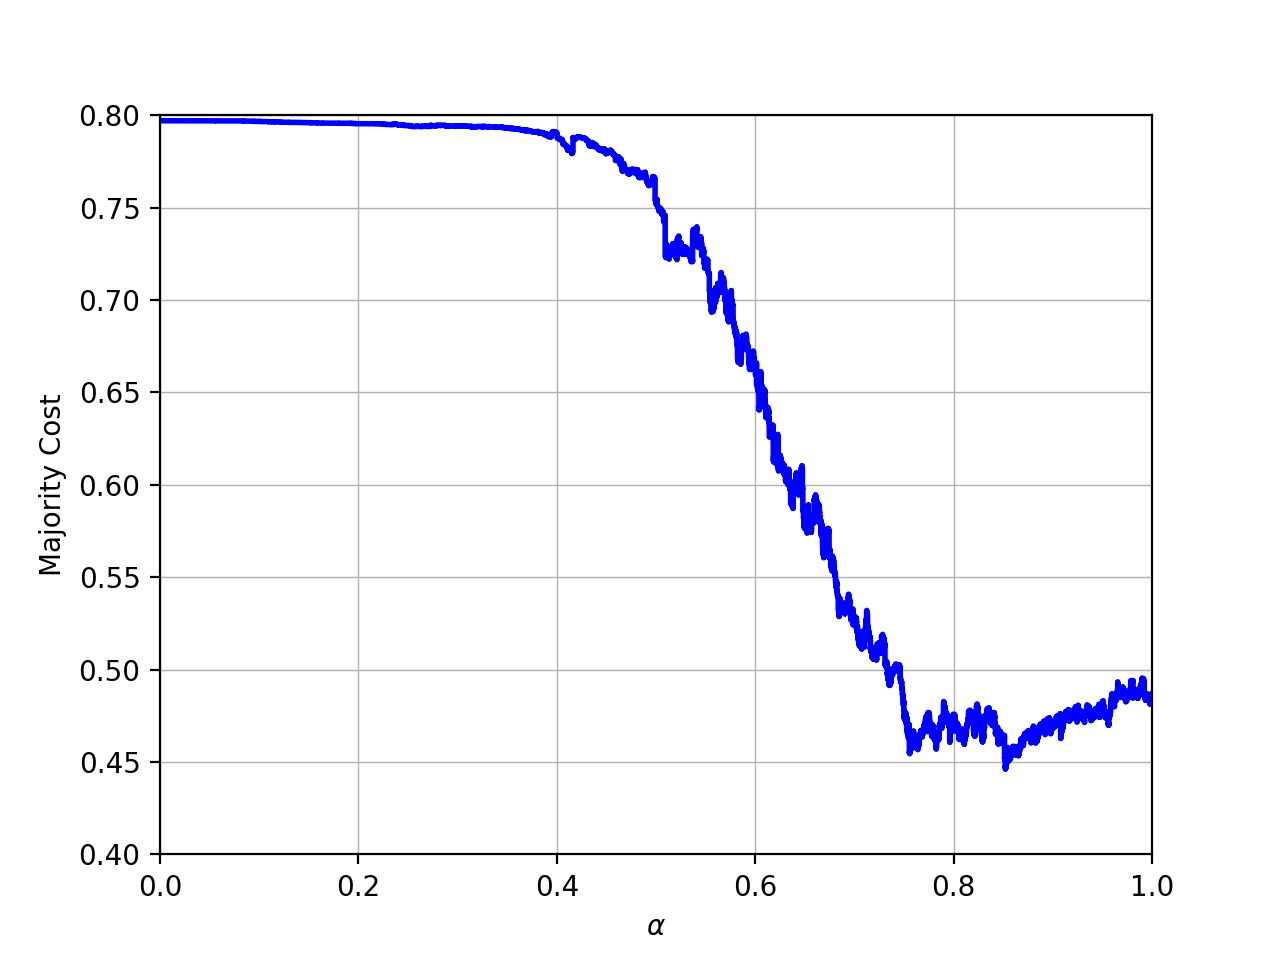
\includegraphics[width=\linewidth]{images/mnist-sc-5}
\end{minipage}
\caption{The first six batches of the MNIST dataset result in similar curves when being evaluated between single and complete linkage.}
\label{fig:mnist1000sc}
\end{figure}

As the curves look quite similar, we also want to analyse if the optimal values are similar. Thus we calculate the hamming cost for the optimal value of $\alpha$ in table \ref{table:mnist1000sc}.

\begin{table}[h]
    \centering
    \begin{tabular}{|l | l l l l l l |}
    \hline
    Strategy & Batch 0 & Batch 1 & Batch 2 & Batch 3 & Batch 4 & Batch 5\\ \hline
    Single Linkage & 0.796901 & 0.797345 & 0.797171 & 0.797405 & 0.796766 & 0.797024\\
    Complete Linkage & 0.490468 & 0.461063 & 0.479825 & 0.475329 & 0.463321 & 0.487111\\
    $\alpha_{opt}$ & 0.87228 & 0.84419 & 0.778498 & 0.83199 & 0.82338 & 0.852251\\
    $cost_{opt}$ & 0.450012 & 0.416433 & 0.431143 & 0.423786 & 0.421103 & 0.446032\\
    $\Delta cost$ & 4.0456\% & 4.463\% & 4.8682\% & 5.1543\% & 4.2218\% & 4.1079\%\\\hline
    \end{tabular}
    \caption{Our proposed algorithm reduces the cost by up to $\Delta_{max} cost = 5.1543\%$.}
    \label{table:mnist1000sc}
\end{table}

We were running the same experiments for the interpolation between average and complete linkage.

\begin{figure}[h]
\centering
\begin{minipage}{.3\textwidth}
  \centering
  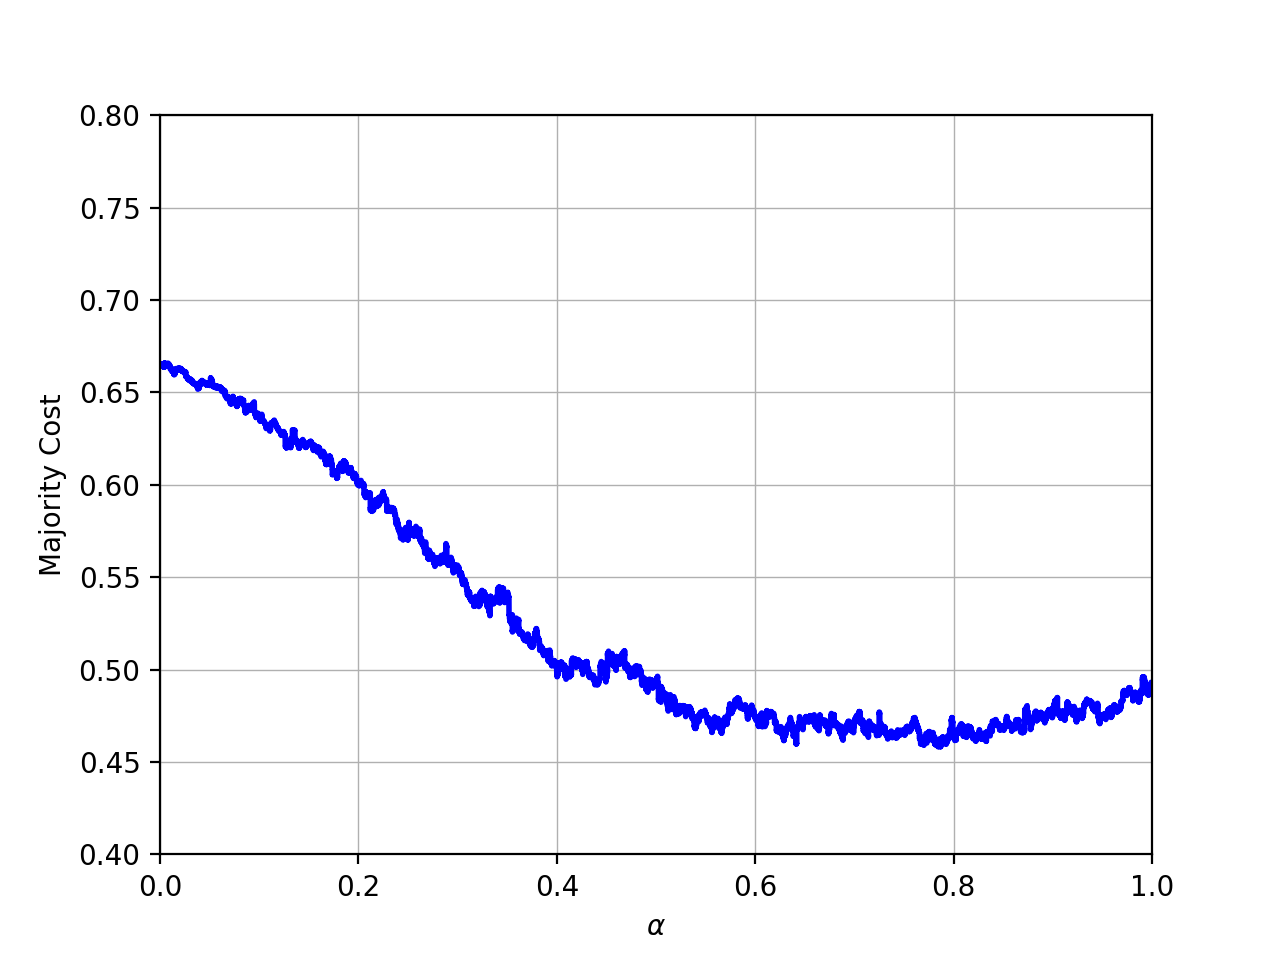
\includegraphics[width=\linewidth]{images/mnist-ac-0}
\end{minipage}
\begin{minipage}{.3\textwidth}
  \centering
  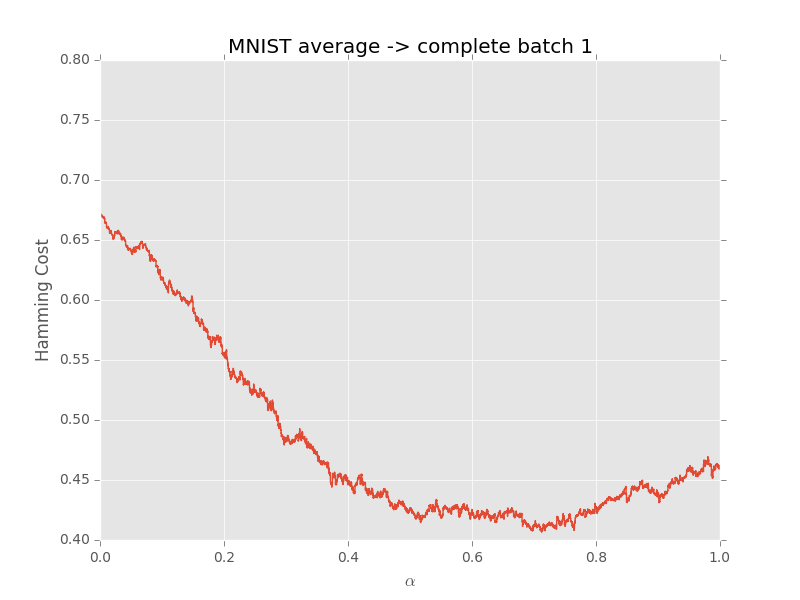
\includegraphics[width=\linewidth]{images/mnist-ac-1}
\end{minipage}
\begin{minipage}{.3\textwidth}
  \centering
  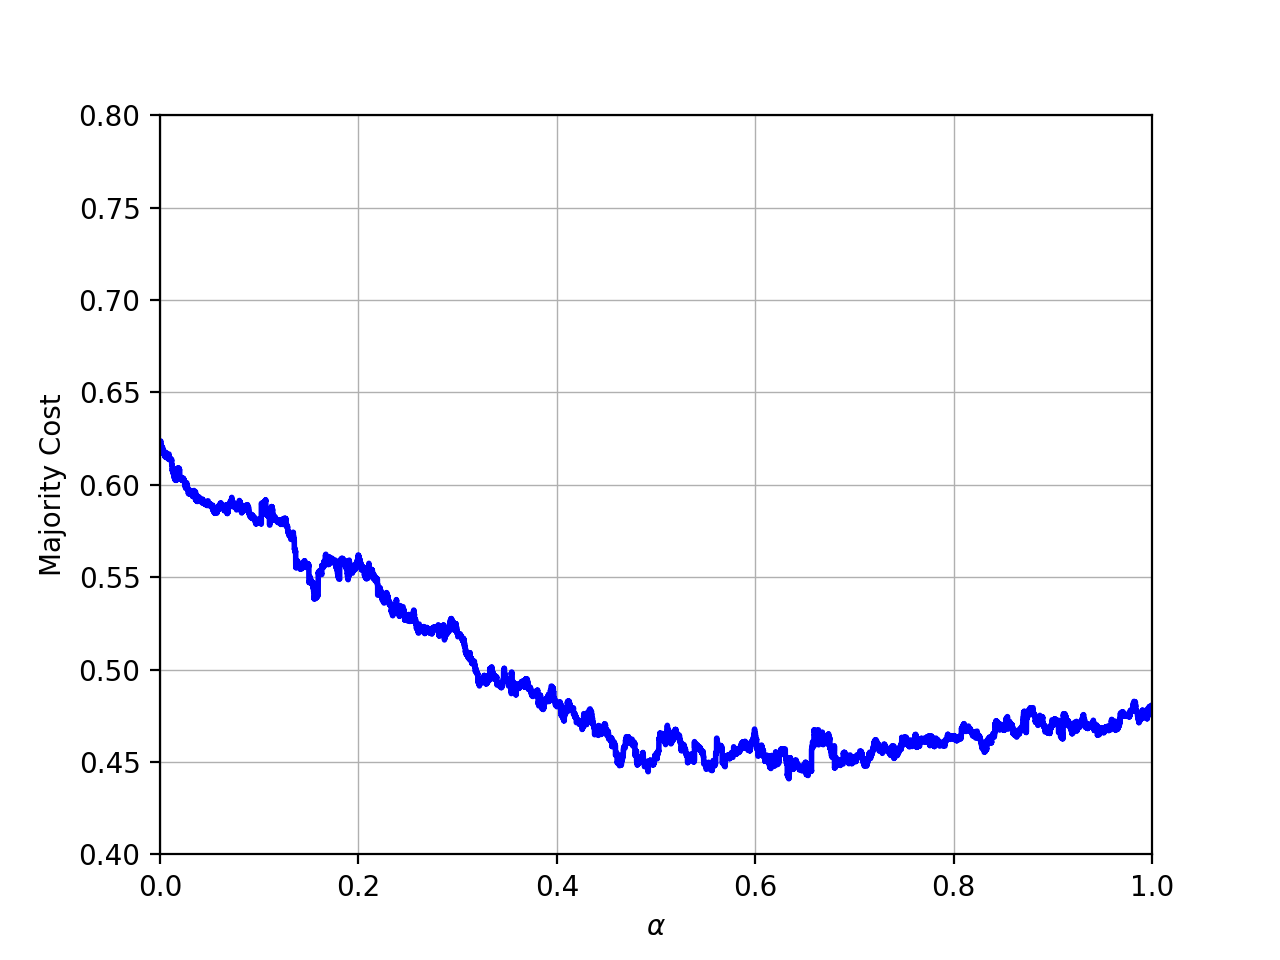
\includegraphics[width=\linewidth]{images/mnist-ac-2}
\end{minipage}
\begin{minipage}{.3\textwidth}
  \centering
  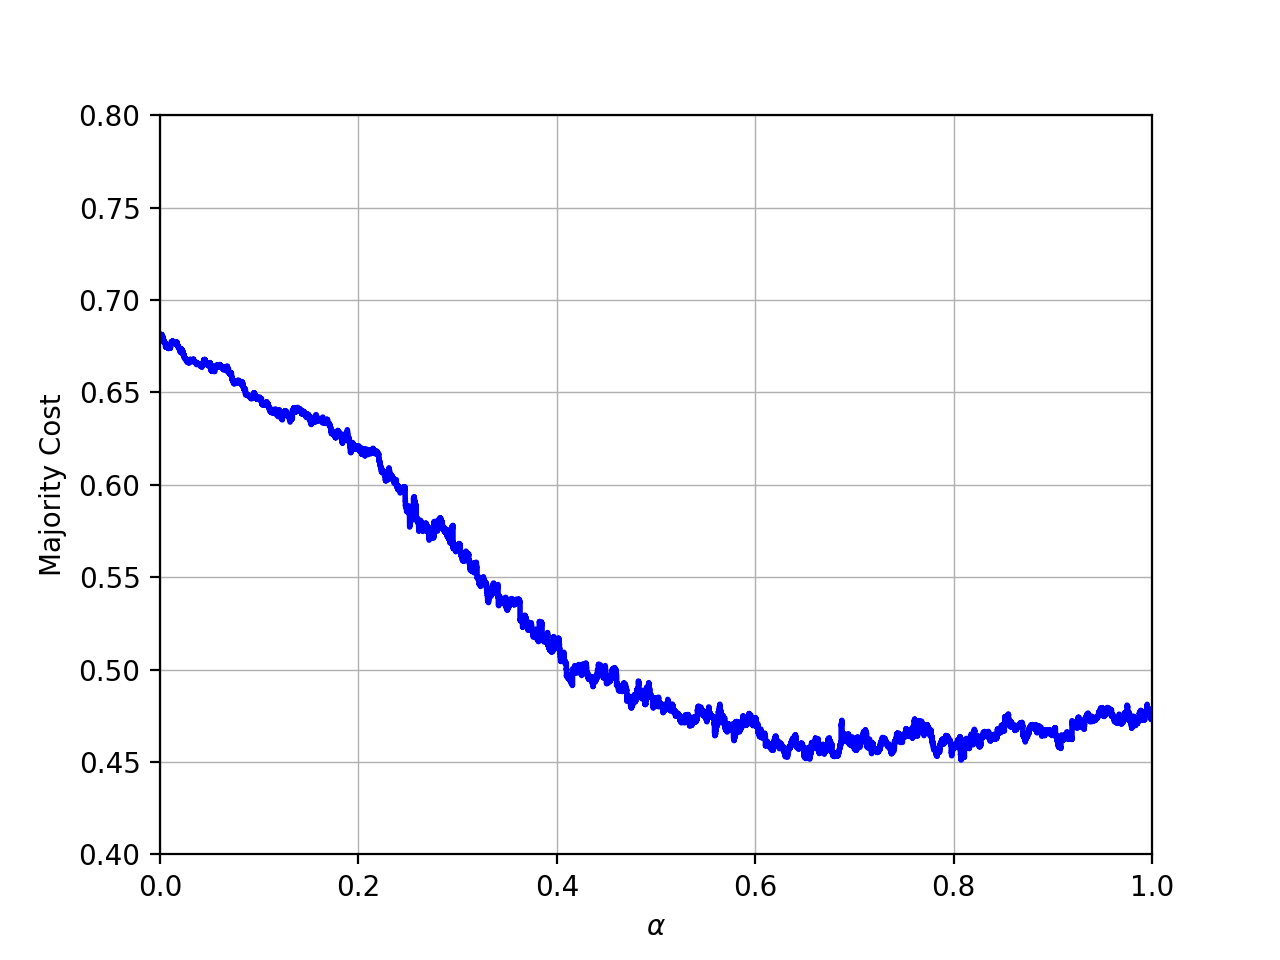
\includegraphics[width=\linewidth]{images/mnist-ac-3}
\end{minipage}
\begin{minipage}{.3\textwidth}
  \centering
  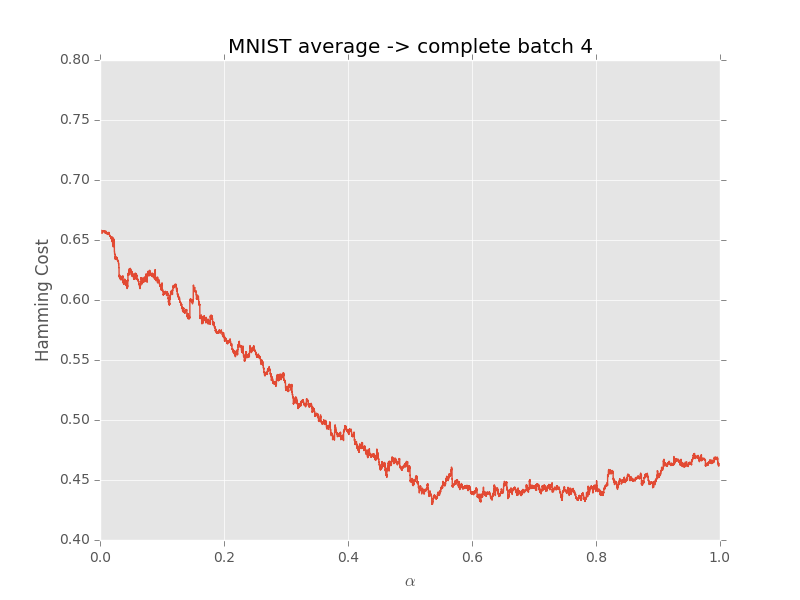
\includegraphics[width=\linewidth]{images/mnist-ac-4}
\end{minipage}
\begin{minipage}{.3\textwidth}
  \centering
  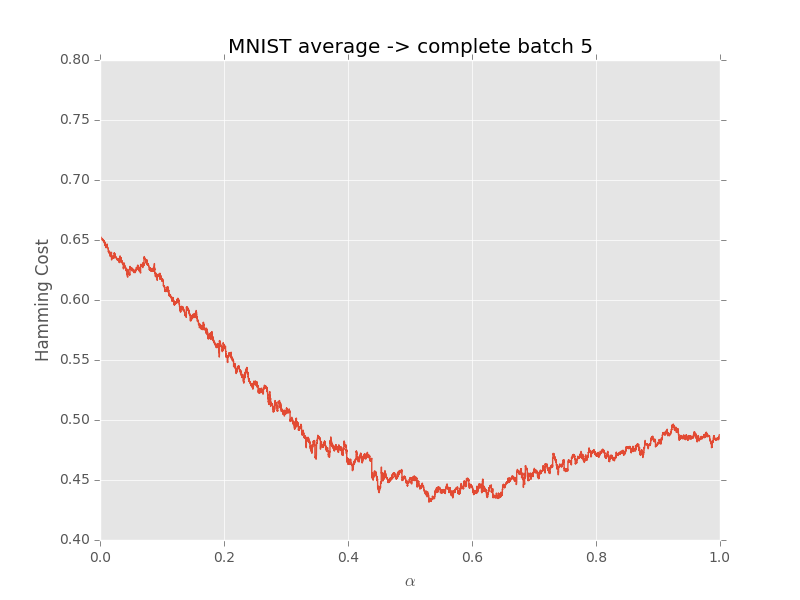
\includegraphics[width=\linewidth]{images/mnist-ac-5}
\end{minipage}
\caption{The omniglot dataset contains handwritten characters of different alphabets, such as Latin, Greek and Hebrew \cite{Lake1332}.}
\label{fig:mnist1000ac}
\end{figure}

\begin{table}[h]
    \centering
    \begin{tabular}{|l | l l l l l l |}
    \hline
    Strategy & Batch 0 & Batch 1 & Batch 2 & Batch 3 & Batch 4 & Batch 5\\ \hline
    Average Linkage & 0.664952 & 0.672583 & 0.623325 & 0.679929 & 0.657857 & 0.652774\\
    Complete Linkage & 0.490468 & 0.461063 & 0.479825 & 0.475329 & 0.463321 & 0.487111\\
    $\alpha_{opt}$ & 0.7869 & 0.7124 & 0.634 & 0.807697 & 0.536073 & 0.5305\\
    $cost_{opt}$ & 0.458167 & 0.406563 & 0.440964 & 0.451063 & 0.429849 & 0.431631\\
    $\Delta cost$ & 3.2301\% & 5.45\% & 3.8861\% & 2.4266\% & 3.3472\% & 5.548\%\\\hline
    \end{tabular}
    \caption{Our proposed algorithm reduces the cost by up to $\Delta_{max} cost = 5.548\%$.}
    \label{table:mnist1000ac}
\end{table}

The curves for interpolating between average and complete linkage in figure \ref{ref:mnist1000ac} vary more than the curves for interpolating between single and complete linkage \ref{fig:mnist1000sc}. This results in a higher variation in the optimal values of $\alpha$ and the performance increase as shown in table \ref{table:mnist1000ac}.

In order to compare the both interpolation strategies, we averaged over the six batches to to see how well the different batches fit to each other. The results are shown in figure \ref{fig:mnist1000avg}.

\begin{figure}[h]
\centering
\begin{minipage}{.45\textwidth}
  \centering
  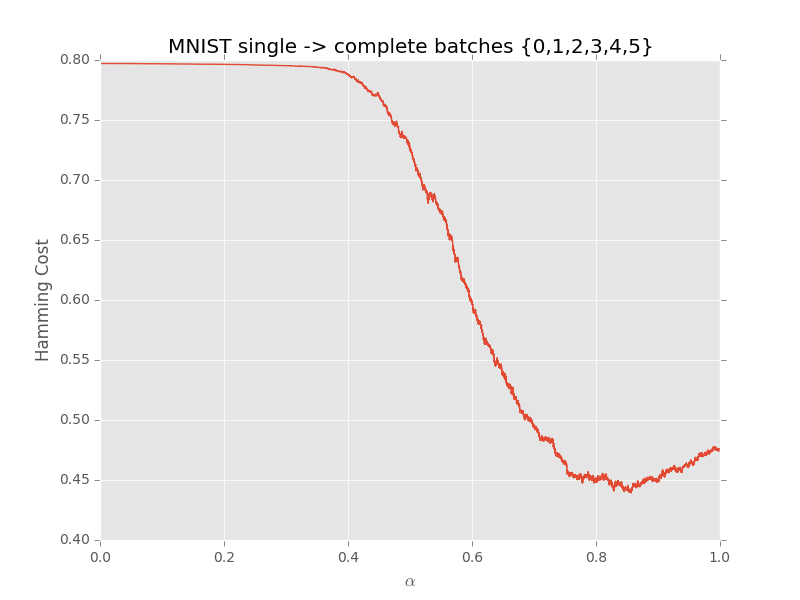
\includegraphics[width=\linewidth]{images/mnist-sc-averaged}
\end{minipage}
\begin{minipage}{.45\textwidth}
  \centering
  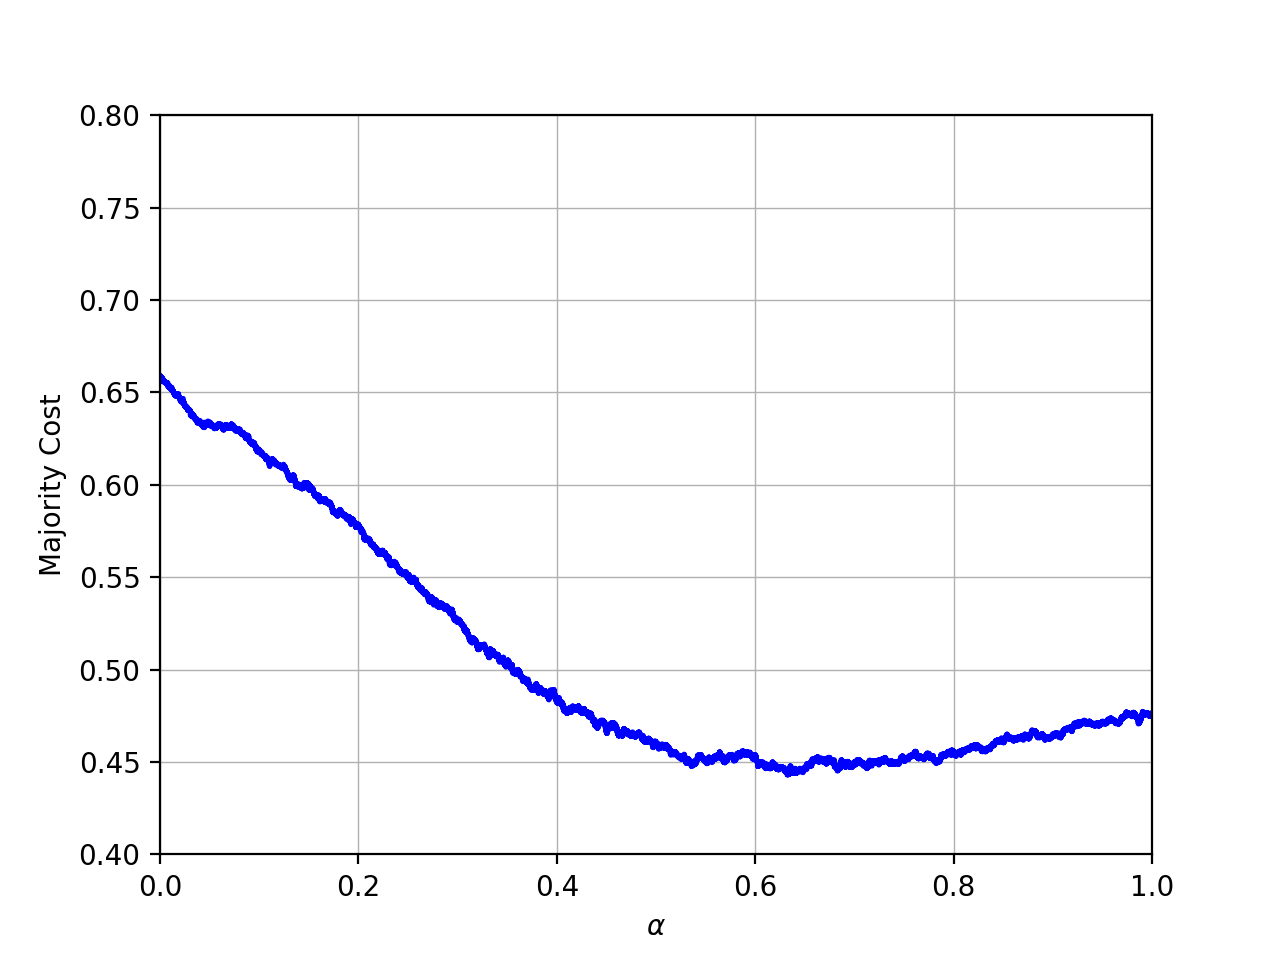
\includegraphics[width=\linewidth]{images/mnist-ac-averaged}
\end{minipage}
\caption{Averaging the first six batches over both linkage strategies allows us to see how good they perform on the first 12,000 points of the MNIST dataset.}
\label{fig:mnist1000avg}
\end{figure}

Figure \ref{fig:mnist1000avg} shows that both strategies give a valuable improvement over single, average and complete linkage on the first 12,000 points of the MNIST dataset. The exact improvement is shown in table \ref{table:mnist1000avg}.

\begin{table}[h]
    \centering
    \begin{tabular}{|l | l |}
    \hline
    Strategy & Hamming Cost\\ \hline
    Single Linkage & 0.797102\\
    Average Linkage & 0.65857\\
    Complete Linkage & 0.476186\\
    $cost_{opt_{SC}}$ & 0.439207\\
    $\Delta cost_{SC}$ & 3.6979\%\\
    $cost_{opt_{AC}}$ & 0.443139\\
    $\Delta cost_{AC}$ & 3.3047\%\\\hline
    \end{tabular}
    \caption{Over the first 12,000 points of the MNIST dataset our algorithm improvese the averaged hamming cost for $3.3\%$ }
    \label{table:mnist1000avg}
\end{table}

Table \ref{table:mnist1000avg} shows that the improvement for average to complete linkage interpolation is $3.3\%$ and for single to complete linkage it is $3.7\%$. The optimal cost corresponds to $\alpha = 0.856557$ in the $SC$ setting and $\alpha = 0.63275$ in the AC setting.

\begin{figure}[h]
\centering
\begin{minipage}{.45\textwidth}
  \centering
  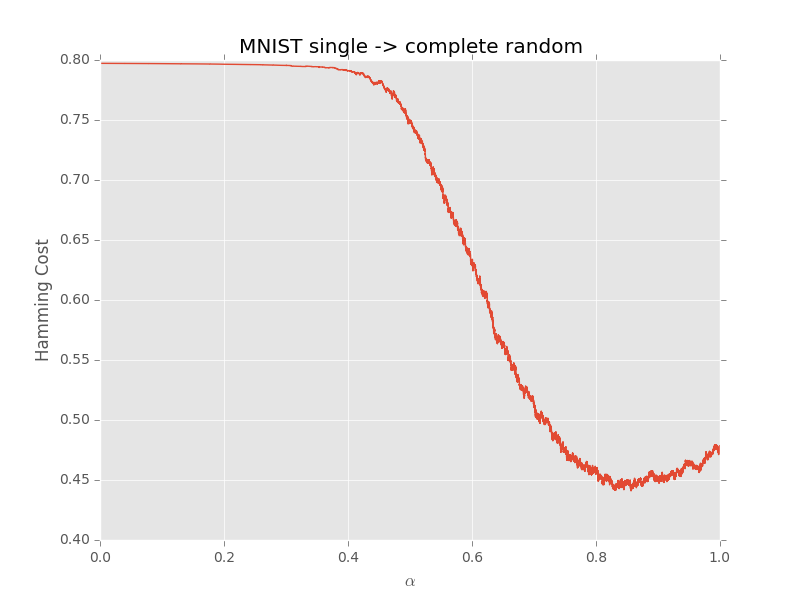
\includegraphics[width=\linewidth]{images/mnist-sc-random}
\end{minipage}
\begin{minipage}{.45\textwidth}
  \centering
  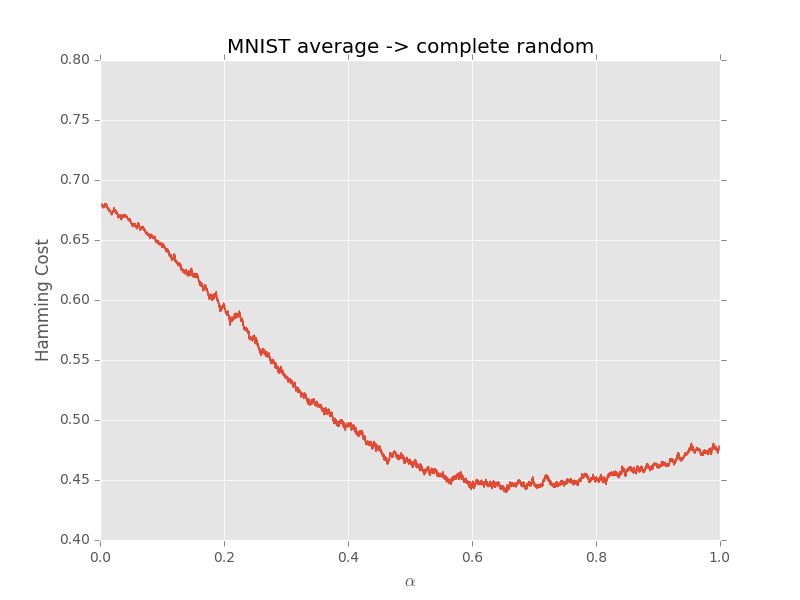
\includegraphics[width=\linewidth]{images/mnist-ac-random}
\end{minipage}
\caption{The first six batches of the MNIST dataset result in similar curves when being evaluated between single and complete linkage.}
\label{fig:mnist1000sc}
\end{figure}

\section{Parameter Advising}

The previously shown results were averaged over multiple experiments and show one parameter $\alpha$ that represents the best clustering over all experiments, i.e. the algorithm automatically outputs the best result. For parameter advising, we select the top $k$ values of $\alpha$ for each experiment and calculate the clustering's cost with the best of the $k$ values of $\alpha$. We select the pool of $\alpha$-values through the local optima for each experiment. The best $k$ values of $\alpha$, where $k$ is much smaller than the number of experiments, can then be calculated with an integer optimization problem. A scenario where this setup can be used is by having a domain expert, who can select the best clustering from the $k$ suggested ones.